Memory effects refer to the influence of historical/past experiences on the perceived video quality. Primacy and recency are two common effects which were investigated in numerous studies \cite{QoEModel_LSTM, QoEModel_TVQoE_ContinuousTimeQoE, QoEModel_NARX_DynamicNetworks}. In addition to these factors, the effect of forgetting curve characteristic and repetition are also considered in our proposed model.
%for the improvement of accuracy
The next parts of this subsection will discuss the role and mathematical function of these factors. Based on that, a memory weight is proposed for the cumulative QoE model.

%/====================================================================================
\subsubsection{Primacy Effect}
%/====================================================================================

The primacy effect \cite{SerialPositionEffect_FreeRecall, PrimacyVsRecency} describes the human behavior to recall (bitrate or rebuffering) initial events occurred at the beginning of the streaming session when providing the overall evaluation \cite{RehearsalProcessesInFreeRecall}. In fact, the primacy effect always exponentially decreases by time \cite{SerialPositionEffect_FreeRecall}. Therefore, its characteristics can be expressed by an exponential curve as follows:
    
\begin{equation} \label{eqn:Primacy}
  f_{P}(t) = exp(-\alpha_{P}*t), \quad 0 \leq t \leq L
\end{equation}
where $\alpha_{P}$ determines the \textit{intensity} of primacy effect (how fast the primacy effect diminishes over time) and $t$ denotes a time instant within a session of $L$ seconds.


%/====================================================================================
\subsubsection{Recency Effect}
%/====================================================================================

The recency effect \cite{SerialPositionEffect_FreeRecall,PrimacyVsRecency} refers to the ability of the human memory to recall the most recent events \cite{RehearsalProcessesInFreeRecall}, hence, the evaluated QoE heavily depends on the recent experiences. The recency effect also can be described by an exponential curve represented by the following equation:
    
\begin{equation} \label{eqn:Recency}
  f_{R}(t) = exp(-\alpha_{R}*(L - t)), \quad 0 \leq t \leq L
\end{equation}
where $\alpha_{R}$ determines the \textit{intensity} of recency effect.
    
The primacy effect and the recency effect can be combined as the U-shaped form \cite{PrimacyVsRecency}, quantifying the influenced weight of the events occurring from the beginning to the end of a video session. As shown in Figure\,\ref{fig:PrimacyRecencyShape}, it can be observed that both Eq. \ref{eqn:Primacy} and Eq. \ref{eqn:Recency} reflect the primacy and recency effect extremely well.
    
\begin{figure}[tb]
  \begin{center}
    \includegraphics[width=0.6\linewidth]{\FigsDir/weight_ideal.png}
  \end{center} 
  \caption{A typical U-shaped curve combined primacy and recency effects.}
  \label{fig:PrimacyRecencyShape}
\end{figure}


%/====================================================================================
\subsubsection{Forgetting Curve and Repetition}\label{pro_for-rep}
%/====================================================================================

\begin{figure}[tb]
  \centering
  \begin{subfigure}[b]{0.49\linewidth}
    \centering
    \includegraphics[width=\linewidth]{\FigsDir/forgetting_curve.png}
    \caption{An example of forgetting curve}
    \label{fig:ForgettingCurve}
  \end{subfigure}
  \hfill
  \begin{subfigure}[b]{0.49\linewidth}
    \centering
    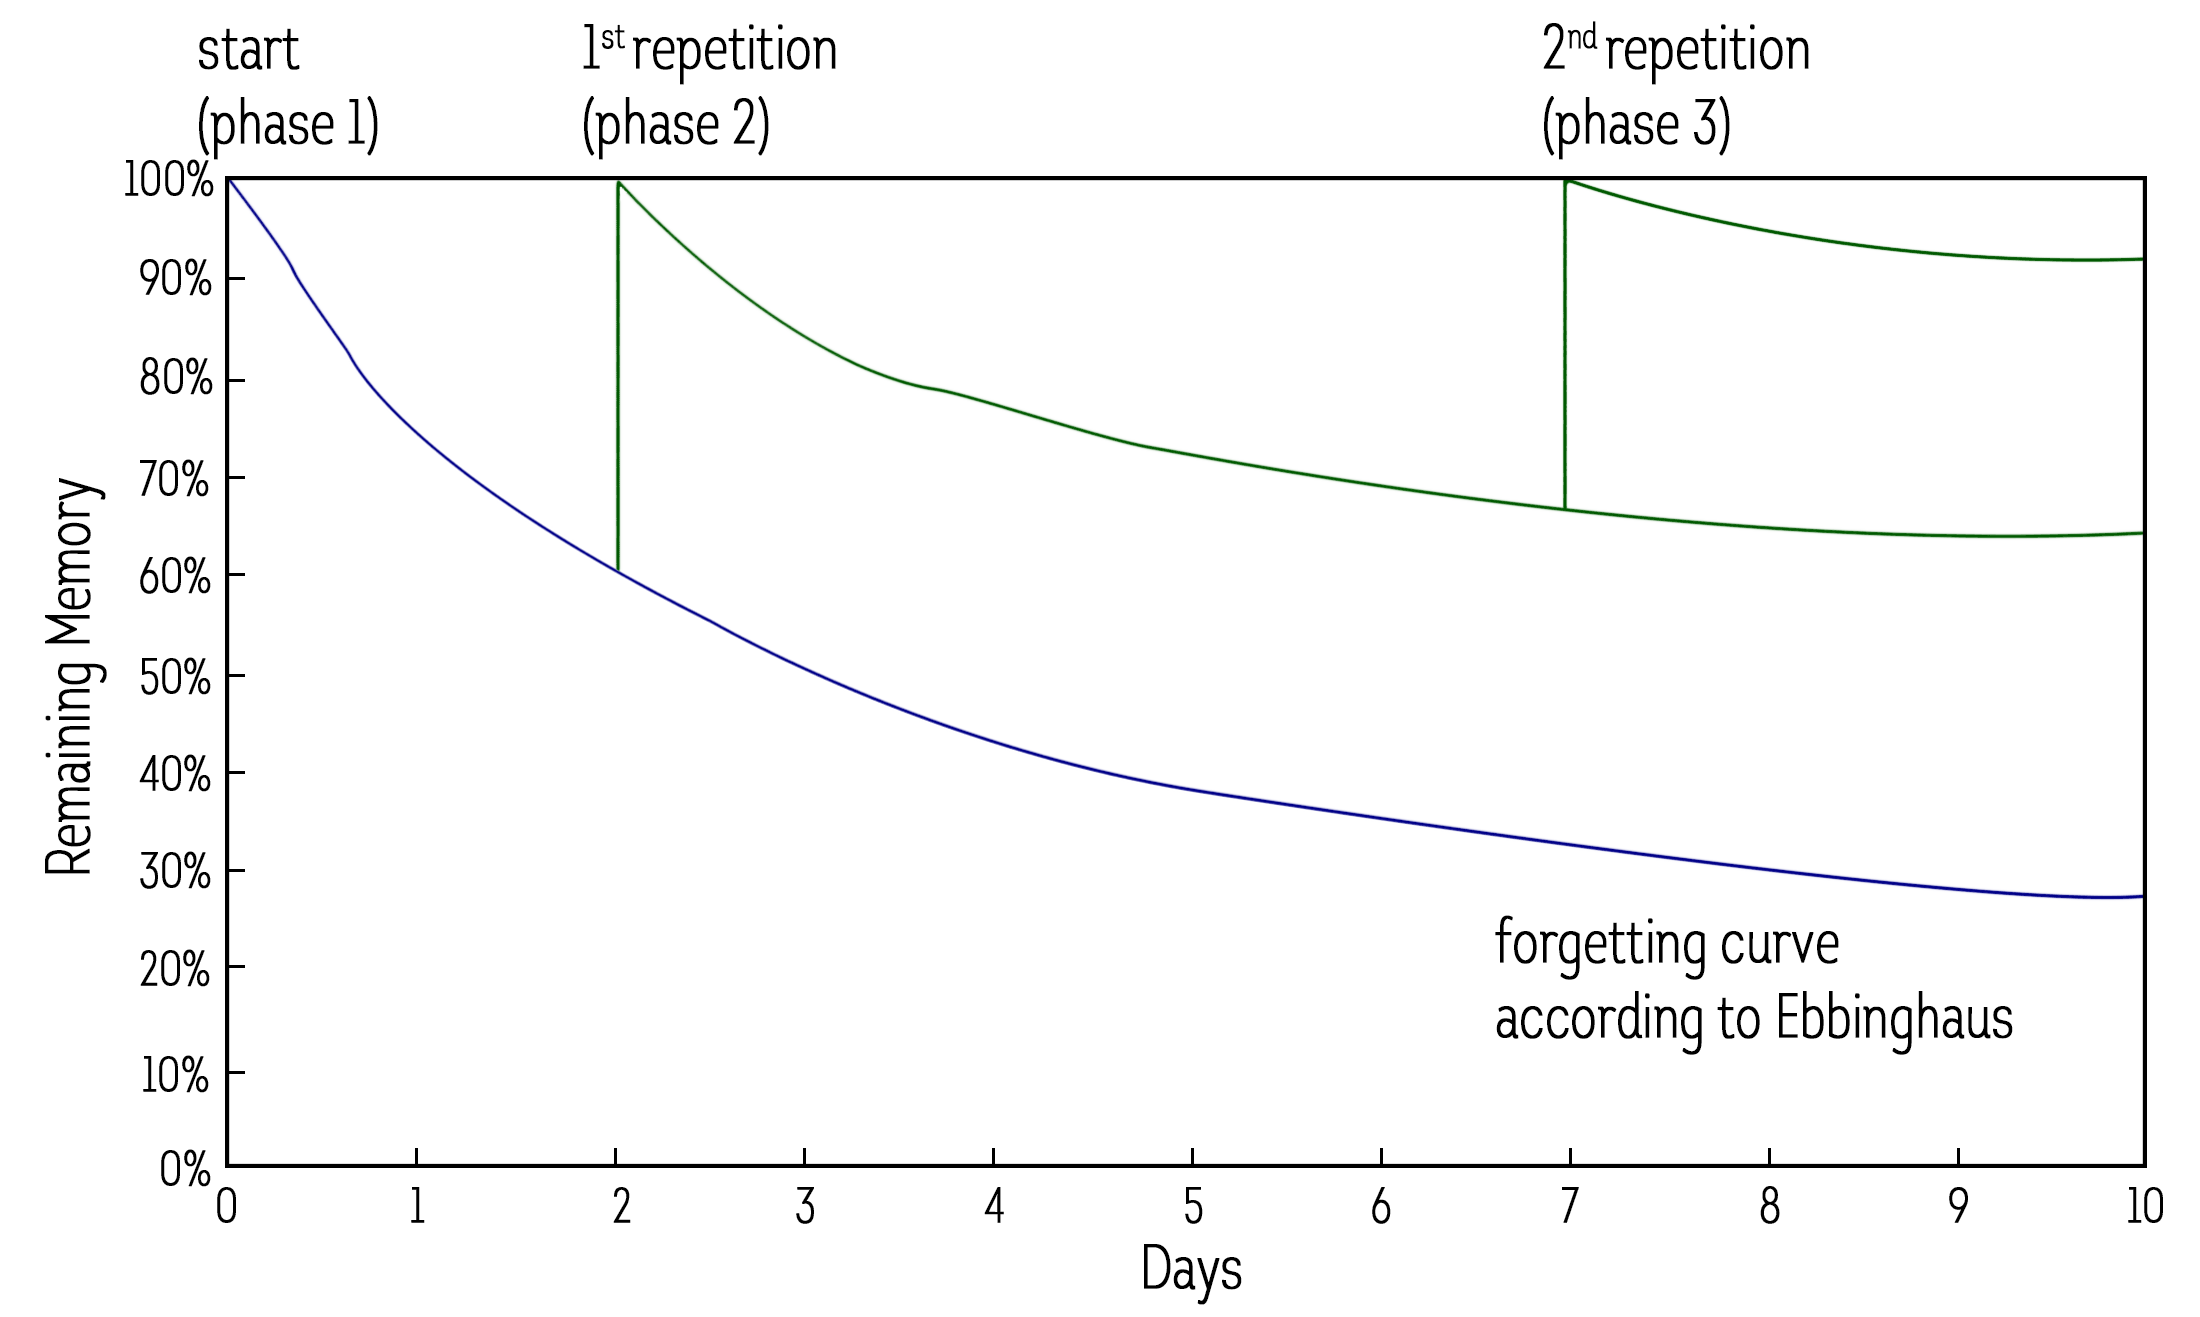
\includegraphics[width=\linewidth]{\FigsDir/repetition_redraw.png}
    \caption{Forgetting curve and repetition}
    \label{fig:ForgettingCurveRepetition}
  \end{subfigure}
  
  \caption{Examples of forgetting curve and repetition.}
  \label{fig:ForgettingCurveRepetitionExamples}
\end{figure}

%Human memory is complex; thus, 
Due to the significant impact of the negative experience caused by distorted events, the primacy and recency effect can be neglected under repeated bitrate switches or rebuffering \cite{EffectSizesOfInfluenceFactors}. In such situations, forgetting behavior and repetition should be taken into account. The forgetting behavior, in other words, forgetting curve characteristic \cite{Ebbinghaus_ForgettingCurve} is a natural process, describing the exponential loss of memory over time. As shown in Figure \ref{fig:ForgettingCurve}, when information is learned, its memory retention declines at an exponential rate. Accordingly, any occurred events can be exponentially forgotten by time if there is no attempt to retain it. The level of remaining memory about such events at a specific time point depends on:

\begin{itemize}
  \item The strength of memory (memory intensity): The durability that memory traces in the brain. The more annoyance the event is, the stronger the user memorizes it and the longer it lasts.
  \item The time has elapsed since the occurrences of events: As shown in Figure\,\ref{fig:ForgettingCurve}, the user will forget an average of 60\% of what they experience within the first period of time \cite{EvaluatingForgettingCurves,Ebbinghaus_ForgettingCurve}.
  \item Repetition: The more frequently an event occurs, the more likely it sticks to the user memory (shown in Figure\,\ref{fig:ForgettingCurveRepetition})
\end{itemize}

In a typical streaming session, an interruption (bitrate switching or rebuffering) can happen regularly. When an event, especially rebuffering repeatedly occurs, the strength of memory of those events will trendily increases \cite{Ebbinghaus_ForgettingCurve}, negatively influencing the perceived video quality. Consequently, as the number of negative events increases, QoE will recover at a slower pace after the occurrence of each event. Such memory characteristics can be formulated as the following equation \cite{TwoComponentsOfMemory}:
    
\begin{equation} \label{eqn:Repetition}
  f_{RP}(t) = exp(-\frac{\alpha_{RP}}{NR(t)} * TR(t)), \quad 0 \leq t \leq L
\end{equation}
where $NR(t)$ is the number of rebuffering events occurring until the time $t$, $TR(t)$ is the time elapsed since the last video impairment, and $\alpha_{RP}$ is the intensity of memory related to a rebuffering event. The ratio $\frac{\alpha_{RP}}{NR(t)}$ determines the retention of the user's memory after the $NR(t)$-th rebuffering. Accordingly, the lower $\frac{\alpha_{RP}}{NR(t)}$ is, the higher retention rate, making $f_{RP}$ declines at a lower rate. 


%/====================================================================================
\subsubsection{Proposed Memory Weight}
%/====================================================================================

As discussed in the previous sub-subsections, the effects of primacy, recency, forgetting behavior and repetition are significantly crucial for the evaluation of the cumulative QoE. Therefore, in the proposed cumulative QoE model, we introduce a novel \textit{memory weight} incorporating the effects of those factors to accurately assess the cumulative human perception during a streaming session. The proposed memory weight is represented by Eq. \ref{eqn:Weight}. An example of time-varying memory weight is illustrated in Figure \ref{fig:ForgettingCurveRebuff}. In fact, Eq. \ref{eqn:Weight} is a linear combination effect of the above-mentioned memory factors obtained from Eq. \ref{eqn:Primacy}, Eq. \ref{eqn:Recency} and Eq. \ref{eqn:Repetition}.
    
\begin{equation} \label{eqn:Weight}
  w_{t} = \beta_{1}f_{P}(t) + \beta_{2}f_{R}(t) + \beta_{3}f_{RP}(t)
\end{equation}

\begin{figure}[tb]
  \begin{center}
    \includegraphics[width=0.7\linewidth]{\FigsDir/weight_different_params.png}
  \end{center} 
  \caption{An example of the memory weight in a session under different values of parameters $\beta_{1}$, $\beta_{2}$, and $\beta_{3}$}
  \label{fig:ForgettingCurveRebuff}
\end{figure}


where $\beta_{1},\beta_{2},\beta_{3}$ respectively determine the contribution of primacy effect, recency effect and repetition to the memory weight.

Figure. \ref{fig:ForgettingCurveRebuff} shows that when an rebuffering event occurs near the end of the session, the recency effect has a stronger effect on human perception. Therefore, in this period of times, the end user's QoE will drops dramatically. In addition, the forgetting rate of a specific interruption is also smaller than those of previous ones, determining the characteristics of forgetting behavior and repetition. Therefore, the proposed memory weight potentially reflects the intensity of human memory over time during a streaming session.
